\documentclass[a4paper,11pt,exos]{nsi} % COMPILE WITH DRAFT
\usepackage{pifont}
\usepackage{fontawesome5}
\usepackage{hyperref}

\begin{document}
\classe{\premiere spé}
\titre{Notion de suite}
\maketitle



On donne les cinq listes de nombres suivantes :
\begin{enumalph}
	\item 	1 ; 4 ; 7 ; 10 ; 13 ; 16 ; 19.
	\item 	1 ; 2 ; 4 ; 8 ; 16 ; 32 ; 64.
	\item	1 ; 4 ; 9 ; 16 ; 25 ; 36 ; 49.
	\item	1 ; 1 ; 2 ; 3 ; 5 ; 8 ; 13 ; 21 ; 34.
	\item	1 ; 11 ; 21 ; 1211 ; 111221 ; 312211 ; 13112221 ; 1113213211.	
\end{enumalph}
\subsection{Des règles de construction}
\begin{enumerate}
	\item 	\textbf{Devinette :} Ces listes ont été construites en suivant des règles de construction précises. Trouver une règle de construction pour chacune.\\
	\textit{Aide :} La suite \textbf{e.} est appelée « look and say sequence ».\\[0.5em]
	\carreauxseyes{16.8}{6.4}
	\item 	\'Ecrire, pour chacune des listes, les quatre termes suivants en utilisant la règle de construction trouvée.\\[0.5em]
	\carreauxseyes{16.8}{6.4}
	\item	Donner le $18^{e}$ terme de chacune des listes \textbf{a, b, c} et \textbf{d}.\\[0.5em]
	\carreauxseyes{16.8}{3.2}
	\item	Peut-on prévoir, pour certaines de ces listes, le $100^{e}$ terme de la liste (sans écrire tous les termes précédents !) ? Si oui, donner sa valeur.\\[0.5em]
	\carreauxseyes{16.8}{4}
\end{enumerate}

\subsection{Une notation}
On note $u_0$ le permier terme d'une liste, $u_1$ le deuxième terme, $u_2$ le troisième terme, etc.
\begin{enumerate}
	\item 	Donner le terme $u_7$ de chaque liste.\\[0.5em]
	\carreauxseyes{16.8}{4.8}
	\item 	On considère une nouvelle liste de nombres $v_0,v_1,v_2$, etc. définie par $\quad v_n=3\times n \quad$ pour tout entier naturel $n$.\\
	\'Ecrire, dans l'ordre, les 8 premiers termes de cette liste.\\[0.5em]
	\carreauxseyes{16.8}{4.8}
\end{enumerate}

\newpage
\subsection{Avec des bâtons}

Avec des bâtons identiques, on réalise les figures suivantes :
\begin{center}
	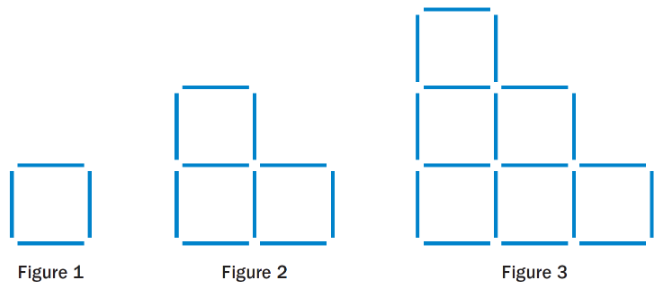
\includegraphics[width=12cm]{batons}
\end{center}
\begin{enumerate}
	\item 	On note $b_n$ le nombre de bâtons nécessaires pour construire la figure $n$, où $n$ est un nombre entier naturel non nul.\\
	De combien de bâtons est composée la figure 5 ?\\[0.5em]
	\carreauxseyes{16.8}{5.6}
	\item 	Proposer une expression de $b_{n+1}$ en fonction de $b_n$.\\[0.5em]
	\carreauxseyes{16.8}{5.6}
\end{enumerate}
\textit{Si besoin, aide au verso.}

\newpage
\textbf{Version guidée :}
\begin{enumerate}
	\item 	
	\begin{enumalph}
		\item 	En utilisant le même procédé de construction, représenter la figure 4.\\[1em]
		
		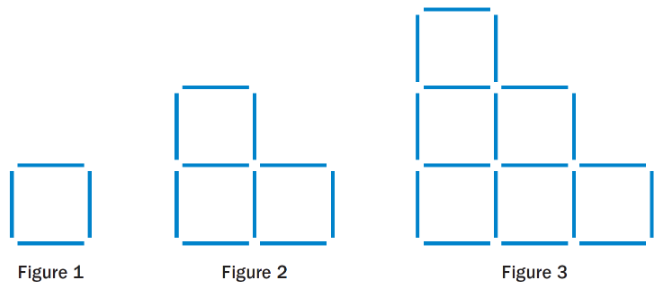
\includegraphics[width=10cm]{batons}
		\item 	Compléter le tableau suivant :
		\begin{center}
			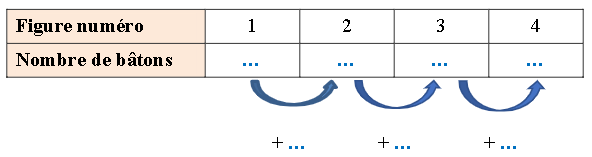
\includegraphics[width=13cm]{tableau}
		\end{center}	
		\item	De combien de bâtons est composée la figure 5 ?\\[0.5em]
		\carreauxseyes{16.8}{5.6}
	\end{enumalph}
	\item 	On note $b_n$ le nombre de bâtons nécessaires pour construire la figure $n$, où $n$ est un nombre entier naturel non nul.
	\begin{enumalph}
		\item 	Compléter les égalités suivantes :
		\begin{multicols}{4}
			$b_2=b_1+...\times 3$
			
			$b_3=b_2+...\times 4$
			
			$b_4=b_3+...\times 5$
			
			$b_5=b_4+...\times 6$
		\end{multicols}
		\item 	Généraliser les égalités précédentes en complétant l'égalité :
		$$b_{n+1}=b_n+...\times(..........)$$
	\end{enumalph}
\end{enumerate}
\end{document}
